\documentclass[conference]{IEEEtran}
\IEEEoverridecommandlockouts
\usepackage[UTF8, scheme=plain]{ctex}
\usepackage{amsmath,amssymb,amsfonts,bm,mathtools}
\usepackage{amsthm}
\usepackage{graphicx}
\usepackage{booktabs}
\usepackage{cite}
\usepackage{hyperref}
\usepackage{tikz}
\usetikzlibrary{arrows.meta,positioning,calc} 
\graphicspath{{../figs/}}
\hypersetup{hidelinks}

\begin{document}

\title{A Filtering-Theoretic Interpretation of Transformers: A State-Space Perspective}

\author{\IEEEauthorblockN{Xiao Yigong, Wang Yun, Wang Kecheng, Huang Niannian, Zhou Changan}
\IEEEauthorblockA{\textit{9XIN AI Research Institute} \\
Sichuan, China \\
xiaoyigong@9xin.ai}
}

\maketitle

\begin{abstract}
This paper presents a theoretical framework that interprets the Transformer architecture through the lens of statistical signal processing. Departing from the conventional sequence modeling perspective, we formulate the self-attention mechanism as a \textbf{non-parametric, data-adaptive filter bank} operating within a learned state space. Specifically, we derive the attention weights from the principle of \textbf{Maximum Likelihood Estimation (MLE)}, characterizing them as instantaneous estimators for \textbf{dynamic Wiener filter} coefficients in non-stationary environments. In this framework, the embedding layer is shown to parameterize the \textbf{underlying state space trajectory} of the physical channel, while the attention mechanism performs \textbf{local statistical estimation} based on the geometric affinity of signal states. Simulation results in \textbf{Acoustic Echo Cancellation (AEC)} scenarios confirm that, even under weak priors, the learned representations spontaneously reconstruct the \textbf{intrinsic geometry} of the physical channel variations (e.g., source trajectories). This correspondence validates the proposed interpretation, bridging the gap between deep learning architectures and classical adaptive filtering theory.
\end{abstract}

\begin{IEEEkeywords}
Transformer, Wiener filtering, non-parametric estimation, state space trajectory, adaptive signal processing
\end{IEEEkeywords}

\section{Introduction}
\IEEEPARstart{I}{n} the realm of statistical signal processing, the optimal estimation of signals in the presence of noise and interference remains a fundamental challenge. For decades, the theoretical foundation of such problems has been dominated by the Linear Time-Invariant (LTI) assumption, under which the classic Wiener-Hopf equation provides a closed-form solution for the optimal filter weights \cite{wiener1949extrapolation}. While computationally elegant, LTI-based methods often fall short in real-world scenarios—such as acoustic echo cancellation (AEC), channel equalization, and clutter suppression—where the system response is inherently non-stationary and exhibits rapid temporal variations.
\subsection{The Challenge of Time-Varying Systems}
To address non-stationarity, adaptive filtering algorithms like the Least Mean Squares (LMS) and Recursive Least Squares (RLS) were developed to track time-varying system responses, denoted as $\mathbf{h}_n$ \cite{haykin2002adaptive, sayed2003fundamentals}. These methods typically rely on a "forgetting factor" or a sliding window to discount past observations, implicitly assuming that the system characteristics remain locally stationary within a short temporal horizon. However, this approach introduces a fundamental trade-off: a short window ensures fast tracking of abrupt changes but suffers from high estimation variance, while a long window reduces noise but introduces lag (bias) during rapid state transitions.
These methods typically rely on a "forgetting factor" or a sliding window to discount past observations, implicitly assuming that the system characteristics remain locally stationary within a short temporal horizon. However, this approach introduces a fundamental trade-off: a short window ensures fast tracking of abrupt changes but suffers from high estimation variance, while a long window reduces noise but introduces lag (bias) during rapid state transitions.
More sophisticated approaches, such as the Kalman filter, explicitly model the evolution of the system via state-space equations \cite{kalman1960new}. While theoretically optimal for linear Gaussian systems, their practical utility is often limited by the requirement of explicit, a priori knowledge of the state transition matrices and noise covariance statistics, which are rarely available in complex, unconstrained physical environments. Consequently, the robust identification of time-varying systems without explicit physical models remains an open problem in the signal processing community.
\subsection{Transformers in Signal Processing}
In recent years, data-driven approaches utilizing Deep Neural Networks (DNNs) have emerged as powerful alternatives to model-based methods. Among these, the Transformer architecture \cite{vaswani2017attention}, originally designed for natural language processing, has demonstrated remarkable performance in various signal processing tasks, including speech enhancement \cite{wang2020complex}, source separation \cite{subakan2021attention}, and nonlinear AEC \cite{zhang2022multi}.
Unlike Recurrent Neural Networks (RNNs) or standard adaptive filters that process data sequentially (and thus suffer from "catastrophic forgetting" of long-term history), the Transformer's self-attention mechanism enables the model to access the entire context window simultaneously. This capability allows for the retrieval of relevant historical information regardless of temporal distance, suggesting an ability to model complex, non-Markovian dynamics. However, despite its empirical success, the Transformer is frequently treated as a "black-box" regressor. A rigorous physical interpretation of \textit{why} the dot-product attention mechanism is effective for signal estimation, and how it relates to established filtering theories, is notably absent in the literature.
\subsection{A Filtering-Theoretic Perspective}
This paper aims to bridge this gap by providing a constructive correspondence between the Transformer architecture and adaptive filtering theory. We posit that the Transformer functions as a \textbf{non-parametric adaptive filter bank} operating on a learned feature manifold.
In our proposed framework, the embedding process is interpreted as a mapping from the observation space to an underlying state space, where the trajectories of the physical system (e.g., the movement of an acoustic source) are disentangled. The attention mechanism, rather than being a heuristic similarity measure, is mathematically formalized as a data-adaptive estimator that computes the posterior probabilities of local statistics. This allows the model to synthesize an instantaneous Wiener solution by aggregating historical states that are statistically coherent with the current query, effectively bypassing the limitations of fixed-window adaptive filters.
This perspective not only offers a physical explanation for the efficacy of Transformers in signal processing tasks but also provides a theoretical basis for designing more interpretable and efficient neural architectures. In the following section, we begin by revisiting the static Wiener solution and extending it to a dynamic, localized estimation formulation, which naturally leads to the attention mechanism.

\section{From Static Solution to Dynamic Localized Estimation}
\label{sec:formulation}

\subsection{Signal Observation Model and Assumptions}
Let us consider a discrete-time signal observation model where the system output $y_n$ is generated by a linear time-varying (LTV) process:
\begin{equation}
y_n = \mathbf{h}_n^T \mathbf{x}_n + s_n + v_n,
\label{eq:obs_model}
\end{equation}
where:
\begin{itemize}
    \item $\mathbf{x}_n \in \mathbb{R}^L$: The observable excitation vector (e.g., reference signal or historical context window);
    \item $\mathbf{h}_n \in \mathbb{R}^L$: The time-varying system impulse response, characterizing the instantaneous causal mapping;
    \item $s_n \in \mathbb{R}$: The latent component of interest (target signal), assumed to be statistically independent of the excitation;
    \item $v_n \in \mathbb{R}$: Random observation noise.
\end{itemize}

This unified model encapsulates a wide range of signal processing and sequence modeling tasks, as summarized in Table~\ref{tab:mapping}.

\begin{table}[htbp]
\centering
\caption{Physical Interpretation of the Signal Model Across Domains}
\label{tab:mapping}
% 调整字号和列间距以适应双栏
\scriptsize 
\setlength{\tabcolsep}{2pt} 
\renewcommand{\arraystretch}{1.2} % 稍微增加行高，防止文字拥挤
% 使用 p{width} 自动换行，总宽度控制在 0.95\columnwidth 以内
\begin{tabular}{@{}p{0.20\columnwidth} p{0.22\columnwidth} p{0.32\columnwidth} p{0.25\columnwidth}@{}}
\toprule
\textbf{Domain} & $\mathbf{x}_n$ (Input) & $\mathbf{h}_n$ (System) & $s_n$ (Target) \\ \midrule
AEC & Ref. Signal & Room Impulse Resp. & Near-end Speech \\
Equalization & Pilot Symbols & Channel Fading & Data Interference \\
Sonar/Radar & Transmit Wave & Clutter Environment & Target Echo \\
Seq. Model & Context Embed. & Semantic Dependency & Residual/ Prediction \\ \bottomrule
\end{tabular}
\end{table}

In this derivation, we impose two fundamental statistical conditions:
\begin{enumerate}
    \item \textbf{Orthogonality of Signal Components}: The excitation and the latent component are uncorrelated:
    \begin{equation}
    \mathbb{E}[x_n s_n] = 0.
    \end{equation}
    \item \textbf{Zero-Mean Noise Condition}: The observation noise satisfies the conditional zero-mean property:
    \begin{equation}
    \mathbb{E}[v_n \mid \mathbf{x}_n] = 0.
    \end{equation}
\end{enumerate}

These conditions ensure that the cross-correlation statistics provide an unbiased estimate of the system response $\mathbf{h}_n$, making the locally weighted least squares (LWLS) solution statistically equivalent to the Maximum A Posteriori (MAP) estimate under Gaussian assumptions \cite{widrow1985}.

\subsection{Dynamic Evolution of the Wiener-Hopf Equation}
In the Maximum Likelihood Estimation (MLE) framework, the static solution relies on global statistics, which fails to capture the time-varying nature of $\mathbf{h}_n$. To address non-stationarity, we assume that the system at any time step $n$ is governed by a latent state $\mathbf{z}_n$, which dictates the local statistical structure but is not directly observable. We therefore introduce an observation-induced state representation:
\begin{equation}
\mathbf{z}_n = \Psi(\mathbf{x}_{1:n}, y_{1:n}),
\label{eq:state_embedding}
\end{equation}
where $\Psi(\cdot)$ denotes an encoding operator that extracts feature representations capturing local statistical coherence from the history $(\mathbf{x}_{1:n}, y_{1:n})$. This concept aligns with Takens' embedding theorem \cite{takens1981}, suggesting that the system's dynamics can be reconstructed in a sufficiently high-dimensional phase space.

We first define the geometric relationship between states. Let the distance metric in the representation space be the squared Euclidean distance:
\begin{equation}
d(\mathbf{z}_n, \mathbf{z}_k) = \|\mathbf{z}_n - \mathbf{z}_k\|^2.
\end{equation}

In statistical physics and kernel methods, distance is often related to an energy function $E(n,k) = d(\mathbf{z}_n, \mathbf{z}_k)$, where lower energy corresponds to higher similarity. Expanding the distance term yields:
\begin{equation}
\|\mathbf{z}_n - \mathbf{z}_k\|^2 = \mathbf{z}_n^T \mathbf{z}_n + \mathbf{z}_k^T \mathbf{z}_k - 2\mathbf{z}_n^T \mathbf{z}_k.
\end{equation}

Since subsequent weighting operations depend only on relative energy differences, terms independent of the comparison target $k$ can be absorbed into scaling factors. We thus introduce a monotonic transformation, expressing "high similarity corresponds to low energy" via an affinity function:
\begin{equation}
\kappa(\mathbf{z}_n, \mathbf{z}_k) \equiv -E(n,k),
\end{equation}
which implies
\begin{equation}
\kappa(\mathbf{z}_n, \mathbf{z}_k) \propto \mathbf{z}_n^T \mathbf{z}_k.
\end{equation}

Consequently, the dot product serves as a proxy for the affinity measure in the representation space. Under this formulation, similar states are expected to share similar statistical structures. We construct a locally weighted likelihood function:
\begin{equation}
J(\mathbf{w}_n) = \sum_{k<n} \alpha_{n,k} (y_k - \mathbf{w}_n^T \mathbf{x}_k)^2 + \beta \|\mathbf{w}_n\|^2,
\label{eq:weighted_likelihood}
\end{equation}
where $\alpha_{n,k}$ represents the unnormalized similarity weights (whose probabilistic form will be derived via the Maximum Entropy principle in the next section), and $\beta$ is a regularization coefficient corresponding to a zero-mean Gaussian prior $p(\mathbf{w}_n) \propto \exp(-\frac{\beta}{2}\|\mathbf{w}_n\|^2)$ on the filter coefficients. This regularization prevents overfitting in finite-sample regimes and ensures the invertibility of the weighted autocorrelation matrix.

Taking the gradient of \eqref{eq:weighted_likelihood} with respect to $\mathbf{w}_n$ and setting it to zero:
\begin{equation}
\frac{\partial J}{\partial \mathbf{w}_n} = -2\sum_{k<n} \alpha_{n,k} \mathbf{x}_k (y_k - \mathbf{w}_n^T \mathbf{x}_k) + 2\beta \mathbf{w}_n = 0.
\end{equation}

Rearranging terms yields the weighted normal equations:
\begin{equation}
\left( \sum_{k<n} \alpha_{n,k} \mathbf{x}_k \mathbf{x}_k^T + \beta \mathbf{I} \right) \mathbf{w}_n = \sum_{k<n} \alpha_{n,k} y_k \mathbf{x}_k.
\label{eq:dynamic_wiener_sol}
\end{equation}

The closed-form solution is given by:
\begin{equation}
\mathbf{w}_n = \mathbf{R}^{-1}(n) \mathbf{P}(n),
\end{equation}
where
\begin{align}
\mathbf{R}(n) &= \sum_{k<n} \alpha_{n,k} \mathbf{x}_k \mathbf{x}_k^T + \beta \mathbf{I}, \\
\mathbf{P}(n) &= \sum_{k<n} \alpha_{n,k} y_k \mathbf{x}_k.
\end{align}

Under the assumption of homoscedastic noise, this weighted least squares solution is equivalent to the conditional expectation estimator. Crucially, the current filter $\mathbf{w}_n$ is determined by local statistics aggregated from historical samples, weighted by their similarity $\alpha_{n,k}$ in the representation space. In this sense, $\mathbf{w}_n$ represents a weighted ensemble of historical experiences most relevant to the current state.

\section{Attention as Non-Parametric Estimation in State Space}
\label{sec:attention_theory}

Having established the dynamic Wiener-Hopf equation \eqref{eq:dynamic_wiener_sol}, the remaining challenge is to determine the optimal form of the similarity weights $\alpha_{n,k}$ and to formalize the statistical role of the attention mechanism. In this section, we derive the scaled dot-product attention from the Maximum Entropy principle and unveil its dual statistical interpretation.

\subsection{Maximum Entropy and the Softmax Kernel}
Let us revisit the relationship between distance and affinity in the representation state space. A natural choice for the similarity weight is the Gaussian kernel:
\begin{equation}
\alpha_{n,k} \propto \exp(-\|\mathbf{z}_n - \mathbf{z}_k\|^2).
\end{equation}
Expanding the squared Euclidean distance yields:
\begin{equation}
\|\mathbf{z}_n - \mathbf{z}_k\|^2 = \mathbf{z}_n^T \mathbf{z}_n + \mathbf{z}_k^T \mathbf{z}_k - 2\mathbf{z}_n^T \mathbf{z}_k.
\end{equation}
When evaluating the relative affinity of a fixed query state $\mathbf{z}_n$ against various historical states $\mathbf{z}_k$, the term $\mathbf{z}_n^T \mathbf{z}_n$ acts as a constant scaling factor. Assuming the state vectors are normalized or vary smoothly in magnitude, the discriminative power of the kernel is overwhelmingly dominated by the inner product. Thus, the unnormalized affinity can be approximated by $E(n,k) \approx -\mathbf{z}_n^T \mathbf{z}_k$.

To translate these deterministic affinities into a valid probability distribution $p(k \mid n)$ for sample selection, we invoke the Maximum Entropy (MaxEnt) principle. Under the constraint that the expected local energy is preserved, the probability distribution that makes the fewest arbitrary assumptions (i.e., maximizes the Shannon entropy) is the Gibbs distribution:
\begin{equation}
p(k \mid n) = \frac{\exp(-\lambda E(n,k))}{\sum_{j<n}\exp(-\lambda E(n,j))}.
\end{equation}
Setting $\lambda = 1$ and substituting the inner product, we obtain:
\begin{equation}
p(k \mid n) = \text{Softmax}\big(\mathbf{z}_n^T \mathbf{z}_k\big).
\end{equation}

In high-dimensional state spaces, the variance of the inner product grows linearly with the dimension $d$. Assuming the features are approximately independent with zero mean and variance $\sigma^2$, we have $\mathrm{Var}(\mathbf{z}_n^T \mathbf{z}_k) \approx d\sigma^4$. To prevent the Softmax function from saturating (which causes vanishing gradients), we introduce a variance normalization factor:
\begin{equation}
\tilde{E}(n,k) = \frac{\mathbf{z}_n^T \mathbf{z}_k}{\sqrt{d}}.
\end{equation}
This normalization ensures that the "temperature" of the Gibbs distribution remains stable across different embedding dimensions. Consequently, the standard scaled dot-product attention \cite{vaswani2017attention} is mathematically recovered as a \textbf{Maximum Entropy posterior of local state similarities}.

\subsection{Dual Statistical Interpretation}
With the attention weights defined probabilistically, we can now unify the Transformer architecture with classical non-parametric estimation theory. 

\newtheorem{theorem}{Theorem}
\begin{theorem}[Dual Statistical Interpretation of Self-Attention]
Under the squared-error loss and the conditional zero-mean noise assumption ($\mathbb{E}[v_n \mid \mathbf{z}_n]=0$), the operation of a single-head attention mechanism can be interpreted as two distinct levels of non-parametric estimation, depending on the definition of the Value projection:
\begin{enumerate}
    \item \textbf{Zero-Order Estimation (Nadaraya-Watson)}: If the Value projection directly maps to the observation $y_k$, the attention output is mathematically equivalent to the Nadaraya-Watson (NW) kernel regression estimator for the conditional expectation $\mathbb{E}[y \mid \mathbf{z}_n]$.
    \item \textbf{First-Order Estimation (Local Linear Weighting)}: If the system follows the dynamic linear model in \eqref{eq:obs_model}, the Softmax-generated weights $p(k \mid n)$ act as the adaptive kernel weights for a Locally Weighted Least Squares (LWLS) problem, thereby inducing the dynamic Wiener filter solution.
\end{enumerate}
\end{theorem}

\begin{proof}
Let the historical dataset be $\{(\mathbf{z}_k, y_k)\}_{k<n}$. The Bayes optimal solution for minimizing the expected risk $\mathbb{E}[(y - f(\mathbf{z}))^2]$ is the conditional expectation $f^\star(\mathbf{z}) = \mathbb{E}[y \mid \mathbf{z}_n]$.

\textit{1) Zero-Order Consistency:} 
The NW estimator approximates this expectation using kernel smoothing:
\begin{equation}
\hat{f}_{\mathrm{NW}}(\mathbf{z}_n) = \frac{\sum_{k<n} K(\mathbf{z}_n, \mathbf{z}_k) y_k}{\sum_{j<n} K(\mathbf{z}_n, \mathbf{z}_j)} = \sum_{k<n} p(k \mid n) y_k.
\end{equation}
By setting the kernel to $K(\mathbf{z}_n, \mathbf{z}_k) = \exp\big(\frac{\mathbf{z}_n^T \mathbf{z}_k}{\sqrt{d}}\big)$ and assigning the Value vector $v_k = y_k$, the attention output $\sum p(k \mid n) v_k$ becomes structurally identical to the NW estimator.

\textit{2) First-Order Extension:} 
When introducing the local linear assumption $y_k \approx \mathbf{w}^T \mathbf{x}_k$, the objective shifts to estimating the time-varying parameter $\mathbf{w}_n$. Under the LWLS criterion:
\begin{equation}
\hat{\mathbf{w}}_n = \arg\min_{\mathbf{w}} \sum_{k<n} p(k \mid n) \|y_k - \mathbf{w}^T \mathbf{x}_k\|^2.
\end{equation}
As derived in \eqref{eq:dynamic_wiener_sol}, the closed-form solution is the dynamic Wiener solution $\mathbf{w}_n = \mathbf{R}^{-1}\mathbf{P}$. 

This proves that the attention mechanism does not merely perform feature aggregation; rather, it provides the statistical weights $p(k \mid n)$ necessary to execute \textbf{non-parametric conditional expectation estimation}.
\end{proof}

\subsection{Physical Implications of the Learned State Space}
The theoretical framework developed above hinges on the encoding operator $\mathbf{z}_n = \Psi(\mathbf{x}_{1:n}, y_{1:n})$. In conventional adaptive filtering, states are either pre-defined (e.g., tapped-delay lines) or explicitly modeled (e.g., Kalman state transitions). In contrast, the Transformer learns $\Psi$ via backpropagation, driven solely by the reconstruction objective.

From a signal processing perspective, $\Psi$ serves as a mapping function that parameterizes the underlying state space of the physical system. By mapping complex, non-stationary temporal sequences into a latent geometric space, the encoder disentangles entangled physical factors (e.g., the spatial trajectory of an acoustic source). Consequently, the highly non-stationary Wiener filtering problem is transformed into a locally stationary, linearly separable problem within this learned state space. The overall data flow and its filtering-theoretic interpretation are summarized in Fig.~\ref{fig:block}.

\begin{figure}[htbp]
\centering
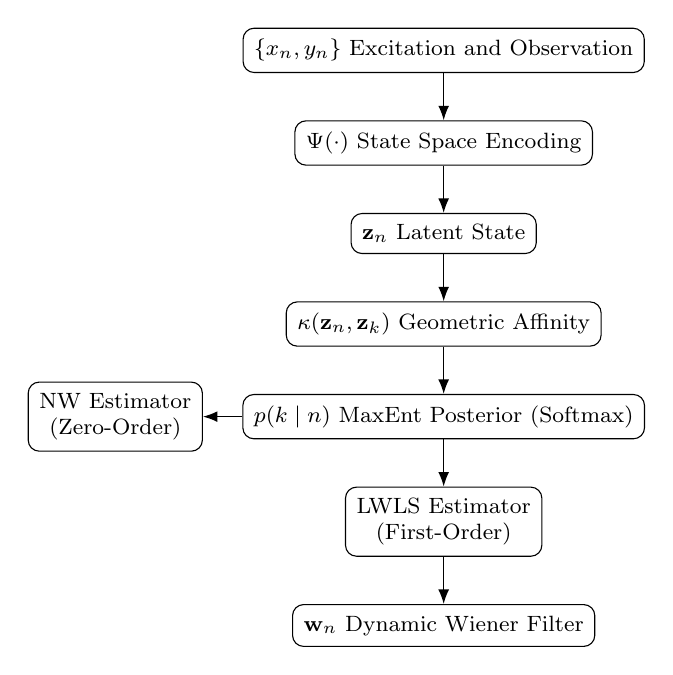
\begin{tikzpicture}[
  node distance=6mm,
  box/.style={draw, rounded corners, align=center, inner sep=4pt, font=\footnotesize},
  arr/.style={-Latex, line width=0.5pt}
]

\node[box] (y) {$\{x_n, y_n\}$ Excitation and Observation};
\node[box, below=of y] (psi) {$\Psi(\cdot)$ State Space Encoding};
\node[box, below=of psi] (z) {$\mathbf{z}_n$ Latent State};
\node[box, below=of z] (kappa) {$\kappa(\mathbf{z}_n,\mathbf{z}_k)$ Geometric Affinity};
\node[box, below=of kappa] (soft) {$p(k \mid n)$ MaxEnt Posterior (Softmax)};

\node[box, left=5mm of soft] (nw) {NW Estimator\\(Zero-Order)};
\node[box, below=of soft] (ls) {LWLS Estimator\\(First-Order)};
\node[box, below=of ls] (w) {$\mathbf{w}_n$ Dynamic Wiener Filter};

\draw[arr] (y) -- (psi);
\draw[arr] (psi) -- (z);
\draw[arr] (z) -- (kappa);
\draw[arr] (kappa) -- (soft);
\draw[arr] (soft) -- (nw);
\draw[arr] (soft) -- (ls);
\draw[arr] (ls) -- (w);

\end{tikzpicture}
\caption{A filtering-theoretic framework of the Transformer architecture. The attention mechanism functions as a local statistical weighting module operating on the learned state space.}
\label{fig:block}
\end{figure}

\section{Simulation and Experimental Validation}
\label{sec:simulation}

\subsection{Experimental Setup and Environment}
To validate the proposed non-parametric adaptive filtering interpretation, we designed a highly non-stationary Acoustic Echo Cancellation (AEC) experiment. The simulation environment was modeled as a $6\text{m} \times 4\text{m}$ rectangular room. A single omnidirectional microphone was placed off-center to eliminate spatial symmetry. To ensure the uniqueness of the physical acoustic fingerprints, we simulated reverberation up to the second-order specular reflections (\text{max-order} $= 2$).

The dataset comprises 15 continuous movement trajectories of the acoustic source, featuring randomized starting points and varied rotational directions (as depicted in the top-right of Fig.~\ref{fig_sim}). This randomization is crucial to breaking any trivial, linear mappings between time steps and physical spatial coordinates. The observable excitation $\mathbf{x}_n$ was defined as a 128-point cross-correlation fingerprint. The training phase employed a self-supervised reconstruction criterion, optimizing solely to minimize the prediction residual without any explicit positional labels.

\begin{figure}[t]
\centering

\includegraphics[width=0.48\textwidth]{simulation_results.png}
\caption{Physical representation capabilities of the Transformer based on multi-trajectory simulations. \textbf{Top Left}: The attention matrix exhibiting strict causal constraints. \textbf{Top Right}: Ground-truth physical trajectories of the acoustic source in Cartesian coordinates. \textbf{Bottom Left}: The theoretical intrinsic geometry of the original acoustic fingerprints (via PCA). \textbf{Bottom Right}: The underlying state space spontaneously reconstructed by the encoder. Color gradients indicate the temporal progression of each trajectory.}
\label{fig_sim}
\end{figure}

% \begin{figure}[t]
% \centering
% 
\includegraphics[width=0.48\textwidth]{training_loss_curve.png}
% \caption{Convergence curve of the training residual. The rapid initial descent corresponds to the establishment of the dominant statistical structure (equivalent to a low-order Wiener solution). The subsequent slow convergence reflects the model's fine-tuning of local statistical coherence within the learned state space. The loss stabilizes at the $10^{-2}$ magnitude with minor oscillations, indicating convergence to a stable local minimum risk estimator rather than mere memorization of the training trajectories.}
% \label{fig_loss}
% \end{figure}

\subsection{Causal Retrieval Properties of the Attention Mechanism}
Fig.~\ref{fig_sim} (top-left) visualizes the causal attention map for a specific batch. Two critical observations emerge:
\begin{enumerate}
    \item \textbf{Causal Boundaries}: The attention matrix exhibits a strict lower-triangular structure, verifying that the causal mask successfully enforces the physical constraint that effects cannot precede their causes.
    \item \textbf{Non-Local Retrieval}: Beyond the localized coherence band along the main diagonal, numerous discrete, off-diagonal bright spots appear. From a physical standpoint, these spots indicate that when the acoustic source moves near a previously visited spatial location, the attention mechanism can bypass long temporal gaps to precisely retrieve historical samples possessing similar second-order statistics. This strongly corroborates that the attention operator functions as a \textbf{content-driven state estimator}, rather than a simplistic temporal smoothing filter.
\end{enumerate}

\subsection{Topological Consistency of the Learned State Space}
A core hypothesis of this paper is that the encoding operator $\Psi$, under the pressure of the reconstruction objective, spontaneously parameterizes the underlying state space of the time-varying channel. We validated this by comparing the intrinsic geometry of the physical signals with the neural representation geometry using Principal Component Analysis (PCA):
\begin{enumerate}
    \item \textbf{Theoretical Intrinsic Geometry (Bottom-Left)}: Direct PCA reduction on the raw cross-correlation vectors reveals the ground-truth topological structure of the Room Impulse Responses (RIRs). It exhibits a distinct, horseshoe-like curved surface.
    \item \textbf{Learned State Space (Bottom-Right)}: This displays the 2D embedding output from the encoder. Remarkably, despite receiving no coordinate supervision during training, the generated representation demonstrates a profound \textbf{topological isomorphism} to the theoretical geometry. Furthermore, the neighborhood relationships among points remain highly continuous with respect to the temporal color gradient.
\end{enumerate}
This morphological isomorphism confirms that the encoding operator successfully achieves an orthogonal disentanglement of coupled physical factors (e.g., the source's radial distance and angular displacement). Consequently, it transforms the highly non-stationary Wiener filtering problem into a locally stationary, linearly separable task within the learned state space.

% \subsection{Performance Evaluation}
% As illustrated in Fig.~\ref{fig_loss}, the training residual converges to below the $10^{-2}$ threshold. During the testing phase, the model successfully outputs smooth state-space coordinates and achieves efficient echo suppression even for unseen, untrained movement trajectories. This generalization capability confirms that the model has internalized the stable physical dynamics of the channel, rather than overfitting to specific data points.

\section{Conclusion and Future Work}
\label{sec:conclusion}

In this paper, we introduced a theoretical framework rooted in statistical estimation to establish a constructive correspondence between the Transformer architecture and dynamic Wiener filtering. We mathematically proved that, under squared-error loss and unbiased observation noise conditions, the attention weights act as a Maximum Entropy posterior distribution within a learned state space. This operation is equivalent to executing a non-parametric local statistical estimation over historical observations. Consequently, the linear projection given by the weighted normal equations corresponds to a local Minimum Mean Square Error (MMSE) estimator.

Through this lens, the Transformer can be unified as a \textbf{non-parametric adaptive filter bank operating on a learned state space}: the Embedding layer parameterizes the system state, Self-Attention performs statistical sample retrieval, and the linear projection executes the locally optimal reconstruction. Acoustic multi-path simulations further demonstrated that, without explicit supervision, the learned representations preserve the topological structure of channel variations and generalize robustly to unobserved trajectories. This implies that the model recovers the low-dimensional dynamics of the underlying physical system instead of merely memorizing temporal sequences.

It is crucial to note that the validity of this interpretation relies on two prerequisites: (1) the statistical independence of the target component and the reference excitation, and (2) the continuity of local statistics within the representation space. Therefore, this theory is particularly suited for causal systems governed by latent state evolution, rather than purely discrete or symbolic random processes. In other words, rather than viewing the Transformer merely as a universal function approximator, our work restricts its definition to a \textbf{state-dependent statistical estimator}.

Looking ahead, this filtering-theoretic perspective opens several promising avenues for future research:
\begin{enumerate}
    \item \textbf{Multi-Head Attention} can be reinterpreted as a set of parallel subspace filter banks, each tracking different statistical sub-bands or scattering multipaths.
    \item \textbf{Positional Encoding} can be viewed as the injection of dynamical priors, implicitly constraining the state transition equations.
    \item \textbf{Diffusion and Sequence Generative Models} might be mapped to stochastic differential estimation processes executing on these learned manifolds.
\end{enumerate}
These directions hold the potential to firmly integrate deep sequence modeling architectures into the unified theoretical framework of stochastic systems and statistical signal processing.

\bibliographystyle{IEEEtran}
\bibliography{../bib/refs.bib} % Your bib file

\end{document}